Ultimately, we will design a deterministic finite automaton (DFA) $M = \langle Q, \Sigma, \delta, q_0, F \rangle$, where $Q$ is the state set, $\Sigma$ is the input alphabet, $\delta : Q\times\Sigma \rightarrow Q$ is the transition function, $q_0$ is the initial state, and $F\subseteq Q$ is the set of final states.

\subsection{Encoding: the alphabet}
\label{sec:overview-alphabet}

First, we define the alphabet $\Sigma$. A finite lattice is represented as a sequence of 5-bit binary strings as described in Figure~\ref{fig:encoding-symbol}. We encode the lattice left-to-right. Note that this means for the first (leftmost) symbol $a=a_0a_1a_2a_3a_4$, it must be the case that $a_0 = a_2 = a_4 = 0$, because edges that correspond to these three symbols do not appear on the lattice.

\begin{figure}
\begin{center}
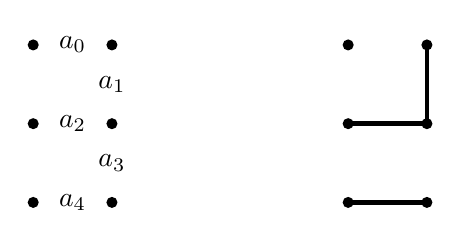
\begin{tikzpicture}
\foreach \x in {0,1}
\foreach \y in {0,1,2}
{
\fill (\x,\y) circle (2pt);
}
\node at (0.5,2) {$a_0$};
\node at (1,1.5) {$a_1$};
\node at (0.5,1) {$a_2$};
\node at (1,0.5) {$a_3$};
\node at (0.5,0) {$a_4$};

\foreach \x in {4,5}
\foreach \y in {0,1,2}
{
\fill (\x,\y) circle (2pt);
}
\draw [ultra thick] (5,2) -- (5,1) -- (4,1);
\draw [ultra thick] (4,0) -- (5,0);
\end{tikzpicture}
\end{center}
\caption{\emph{Left:} Positions of each of 5 bits in the binary string $a = a_0a_1a_2a_3a_4$, a symbol in the alphabet; $a_i = 1$ if there is an edge in position $a_i$, and 0 otherwise. \emph{Right:} Example input symbol $a=01101$ as it appears on the lattice.}
\label{fig:encoding-symbol}
\end{figure}

\subsection{State}
\label{sec:overview-state}

The finite automaton reads input symbols over the alphabet described in Section~\ref{sec:overview-alphabet}, and determines if they represent a valid self-avoiding walk as defined in Section~\ref{sec:statement}. A state in this automaton is represented by a 4-tuple $q = \langle t, m, b, c\rangle$:
\begin{itemize}
\item Elements $t$, $m$, and $b$ represent the degrees of the top, middle, and bottom (respectively) of the rightmost vertices of the input so far. (Notice that these values depend only on the most recent input symbol.) Because self-avoiding walks do not have branches, we are only interested in states for which $t, m, b \in \{0, 1, 2\}$. Provided the input is a valid walk, the number of ones among $t$, $m$, and $b$ represents the number of vertices that the next input symbol may connect to. We divide states by this characteristic:
\begin{itemize}
\item If a state has a single 1-degree vertex, then we refer to it as \emph{single-ended}.
\item If a state has exactly two 1-degree vertices, then we refer to it as \emph{double-ended}. Notice that if we are in a double-ended state, we must have already seen both ends of the valid walk (because one end is at the origin and to induce a second would otherwise require a branch, which is not allowed).
\item If a state has three 1-degree vertices, then we refer to it as \emph{triple-ended}. For the purpose of identifying closed loops, we require an additional bit of state in the case of triple-ended states because two possible pairs of states may have already been connected; see the description of the $c$ element.
\item If a state has no 1-degree vertices, then we have finished processing the walk and any further input should be trivial in order for the lattice to be valid.
\end{itemize}
\item Element $c$ represents closure information. If the state is single- or double-ended, then $c$ is not needed (so $c=0$ in those cases); if the state is triple-ended, $c$ will be either 1 or 2 depending on which pair of vertices is connected:
\begin{itemize}
\item If the middle and bottom vertices are connected, then $c=1$.
\item If the top and middle vertices are connected, then $c=2$.
\end{itemize}
\end{itemize}

In addition to the states that can be described in the manner outlined above, we will use three auxilliary states: \emph{`start'}, \emph{`done'}, and \emph{`dead'}. We present the complete state set $Q$ in Table~\ref{tab:states}.

\begin{table}
\begin{center}
\begin{tabular}{cccc}
\hline
Single-ended & Double-ended & Triple-ended & Auxilliary \\
\hline
1000 & 1010 & 1111 & \emph{start} \\
1200 & 1210 & 1112 & \emph{done} \\
1220 & 1100 &  & \emph{dead} \\
0100 & 1120 &  &  \\
2100 & 0110 &  &  \\
0120 & 2110 &  &  \\
0010 &  &  &  \\
0210 &  &  &  \\
2210 &  &  &  \\
\hline
\end{tabular}
\end{center}
\caption{The state set $Q$, categorized by how many 1-degree vertices there are in the set of rightmost vertices. Final states include all the single-ended states, as well as the \emph{`start'} (accept walks of length 0), and \emph{`done'} states. (The delta function outlined in Section~\ref{sec:overview-delta} may be used to verify that every state listed here is reachable from the start state.)}
\label{tab:states}
\end{table}

\subsection{Transition function}
\label{sec:overview-delta}

In this section, we present an overview of the algorithm behind the transition function $\delta$. For the implementation details, see Section~\ref{sec:implementation}.

There are only a four valid inputs for the first input symbol (because only two edges represented actually appear on the lattice); furthermore, because we require that walks start at the origin, we must ensure that there is no more than one edge connected to that vertex. Therefore, we first handle the case that the input state is \emph{`start'} by handling each of the four inputs directly.

At this point, we should decide where to transition on trivial input (i.e.\ the input is $a=00000$). From an accepting state (\emph{`done'} or any single-ended state), there should be a transition to the \emph{`done'} state; on trivial input from any non-accepting state, there should be a transition to the \emph{`dead'} state.

The \emph{`dead'} state is just that: dead; so it has a self-loop on any input.

Now consider the would-be next state $q'=\langle t', m', b', c' \rangle$. Calculating $t'$, $m'$, and $b'$ is straightforward, as these are only dependent on the input symbol. If these values indicate that the next state will \emph{not} be a triple-ended state, then we may set $c'=0$. If $t'=m'=b'=1$, then we could be in a triple-ended state, so we need to set $c'$ to 1 or 2 based on the criterion described in Section~\ref{sec:overview-state}. If $q$ is a triple-ended state, then the connectedness of $q'$ is the same as that of $q$, so $c'=c$ (this is because connectedness cannot switch between two triple-ended states without an intermediate single-ended state). If $q$ is a single-ended state, then the connectedness of $q'$ depends on which vertex corresponds to the original walk.

Once the possible next state $q'$ has been calculated, we need to check that the lattice could still contain a valid self-avoiding walk. We check several conditions that, if satisfied, will result in a transition to a dead state. These are enumerated in the order that we check them below.
\begin{enumerate}
\item Check for a ``branch''. Calculate the new degree for vertices of $q$ \emph{including} current input. If any of these vertices or any vertex of $q'$ has degree higher than 2, transition to the \emph{`dead'} state.
\item Check for a ``horizontal jump''. Given input $a=a_0a_1a_2a_3a_4$, if $a_0 = a_2 = a_4 = 0$, but at least one of $a_1$ and $a_3$ is 1, then transition to the \emph{`dead'} state.
\item At any point while processing a valid input lattice (if we have not yet reached the \emph{`done'} state), there will be a single degree-1 vertex (an ``end'') that is connected to the origin. The ``vertical jump'' case is characterized by an input that renders this running path unreachable. To check for this, we consider three separate cases:
\begin{itemize}
\item If $q$ is single-ended, then check that its degree-1 vertex connects to the input symbol. If it does not, transition to the \emph{`dead'} state. 
\item If $q$ is double-ended, then check that \emph{}
\item 
\end{itemize}
\end{enumerate}
